%  path0 <- "c:/data/NameRight/"; setwd(path <- paste0(path0, "program/"));  system("recycle c:/data/NameRight/program/cache/ReadData/"); library(knitr); knit("ReadData.rnw", "ReadData.tex"); system("platex ReadData"); system("pbibtex ReadData"); system("dvipdfmx ReadData")

\input{c:/migrate/R/knitrPreamble/knitr_preamble.rnw}
\renewcommand\Routcolor{\color{gray30}}
\makeatletter
\g@addto@macro{\UrlBreaks}{\UrlOrds}
\newcommand\gobblepars{%
    \@ifnextchar\par%
        {\expandafter\gobblepars\@gobble}%
        {}}
\makeatother
\def\pgfsysdriver{pgfsys-dvipdfm.def}
\usepackage{tikz}
\usetikzlibrary{calc, arrows, decorations, decorations.pathreplacing, backgrounds}
\usepackage{adjustbox}
\usepackage{longtable}
\usepackage{caption}
\tikzstyle{toprow} =
[
top color = gray!20, bottom color = gray!50, thick
]
\tikzstyle{maintable} =
[
top color = blue!1, bottom color = blue!20, draw = white
%top color = green!1, bottom color = green!20, draw = white
]
\tikzset{
%Define standard arrow tip
>=stealth',
%Define style for different line styles
help lines/.style={dashed, thick},
axis/.style={<->},
important line/.style={thick},
connection/.style={thick, dotted},
}


\begin{document}
\setlength{\baselineskip}{12pt}





\hfil Read cleaned NBER files\\

\hfil\MonthDY\\
\hfil{\footnotesize\currenttime}\\
\renewcommand{\thefootnote}{*\arabic{footnote}}

\hfil Seiro Ito

\setcounter{tocdepth}{3}
\tableofcontents

\setlength{\parindent}{1em}
\vspace{2ex}


\section{Read files}


NHGIS (IPUMS) has marriage related data sets. 


NBER has a project that compiled marriage data between 1968-1988 {\footnotesize (\url{https://www.nber.org/research/data/marriage-and-divorce-data-1968-1995-0})}.



Create state names in divorce and marriage data with a reference to marr88.pdf. \textsf{StNum} in usst data is \textsf{state} in divorce data.


\subsection{Plots}




\mpage{\textwidth}{
\hfil\textsc{Figure \refstepcounter{figure}\thefigure: Number of marriages by state (NBER)\label{NBER marriage}}\\
\hfil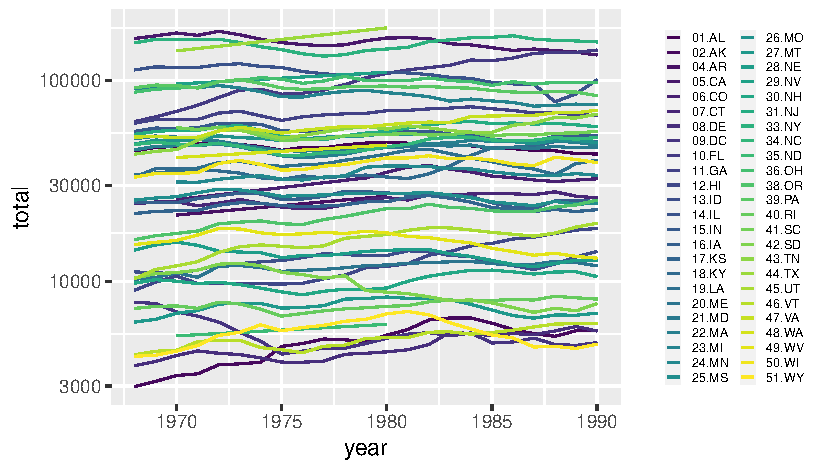
\includegraphics[width=12cm]{c:/data/NameRight/save/NumberOfMarriagesByState.pdf}
}

\mpage{\textwidth}{
\hfil\textsc{Figure \refstepcounter{figure}\thefigure: Number of divorces by state (NBER)\label{NBER marriage}}\\
\hfil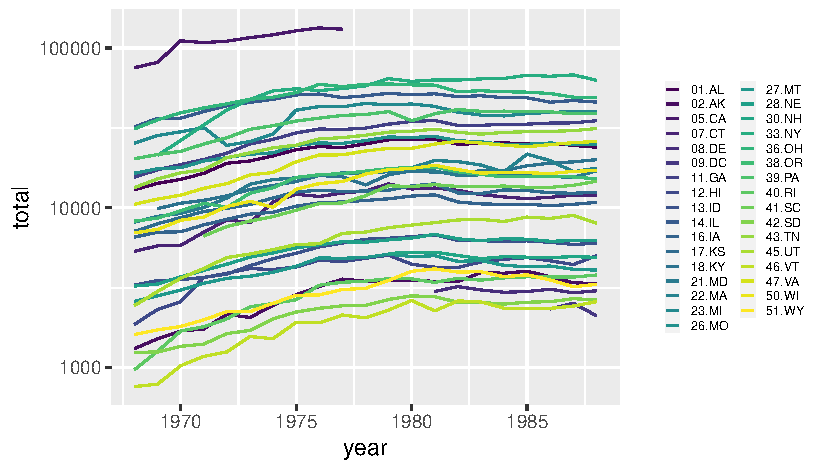
\includegraphics[width=12cm]{c:/data/NameRight/save/NumberOfDivorcesByState.pdf}
}


\section{Legal cases and political activities}


By 1971, Department of State's position: ``[t]he legal name of a married woman is her husband's surname.'' In addition, to quote from \textit{Walker v. Jackson}, 391 F. Supp. 1395 (E.D. Ark. 1975), 
\begin{quotation}
[T]he Supreme Court of the United States has recognized that a State may constitutionally require a married woman to use her husband's surname as her own for certain purposes, as for example obtaining a driver's license, if the State has a sufficiently compelling interest in imposing the requirement. \textit{Forbush v. Wallace}, Governor, 405 U.S. 970, 92 S. Ct. 1197, 31 L. Ed. 2d 246 (1972), aff'g without opinion, \textit{Forbush v. Wallace}, Governor, 341 F. Supp. 217 (M.D.Ala.1971).
\end{quotation}
Such a position in public offices have slowly changed. According to \citet[][p.6]{Augustine1997}, legal challenges in the 1970's ``firmly establised that ... her name is unchanged by the fact that marriage had occurred.'' ``By the late 1970's and early 1980's many state legislatures codified a woman's right to name herself.'' 

The leading case was \textit{Dunn v. Palermo} in Tennessee (1975) that the State Supreme Court affirmed that women can register to vote under her maiden names. Additionally, in 1976, Florida District Court of Appeals noted that women are not compelled to change her name upon marriage (\textit{Marshall v. State}). Another leading case that recognizes the women's right to name is in Nebraska in 1978 (\textit{Simmons v. O'Brien}). In this case, the woman retained her former surnames during the marriage, then filed a divorce (marriage dissolution) to which the District Court denied the appeal because she did not file under husband's surname. The Trial Court reversed the District Court's decision and remanded with directions to accept the filing.

Other scholar notes that a 1973 case in Maryland (\textit{Stuart v. Bd. of Supervisors of Elections for Howard County}) served as a guide, and a 1975 decision in Wisconsin (\textit{Kruzel v. Podell}) played a pivotal role across the US \citep[][fn 4]{MacDougall1985}. \textsc{Table \ref{TabMFn9}} lists all the formal cases and informal opinions by state judicial or state attorney generals affirming the right after 1972. In principle, one can date the year when the official common law practice shifted to affirm the right.\footnote{\href{https://law.justia.com/cases/federal/district-courts/FSupp/406/359/2143469/}{\textit{Allen v. Lovejoy}}, concluded in October 1975, however, notes that a woman who was suspended without pay due to noncompliance with Health Department's name change policy should not get compensation because she did not follow Department's advice to first change the name and appeal to the internal Merit System Council. Given the uncertainty of how MSC might have responded to plaintiff's appeal, the women's name right had not been fully protected until 1974 when the suspension was decided. } 


Following is a summary of political activities that promote women's name rights \citep[][fn 5]{MacDougall1985}: 
\begin{itemize}
\vspace{1.0ex}\setlength{\itemsep}{1.0ex}\setlength{\baselineskip}{12pt}
\item	The Center for a Woman's Own Name was established in 1973 after \textit{Kruzel v. Podell} case was appealed, and started distributing \textit{Booklet For Women Who Wish To Determine Their Own Names After Marriage}. 
\item	In 1974, Olympia Brown League was formed to aid women in Milwaukee affected by the lower court's ruling. In 1972, Massachusetts women formed Name-Change at the time of \textit{Forbush} case\footnote{\textit{Forbush v. Wallace} (1972): A supreme court case that conceded that a woman's legal name is her husband's name. }. They also distributed a booklet titled \textit{Fact Sheet For Women Who Wish To Retain Their Own Name After Marriage}. 
\item	In 1973, \textit{the Committee To Encourage Richard H. Austin To Give Michigan Women Their Middle Names For The Holidays (CERHA)} was formed with Attorney Jean L. King to support the right of women to obtain drivers' licenses using their birth names as middle names. 
\item	In California, \textit{the Name Choice Center} distributed a fact sheet and promoted the issue with the Attorney General and the Legislature. The Center had a mailing list of over 15,000 by 1974. 
\item	In 1974, \textit{The Women's Legal Defense Fund} in Washington, D.C. established a committee
on names which published and distributed a booklet on women's names for D.C. area residents. 
\end{itemize}


\begin{Schunk}
\begin{Soutput}
   state          case                            reference year
1: Texas Rice v. State 37 Tex. Crim. 36, 38 S.W. 801 (1897) 1897
\end{Soutput}
\end{Schunk}




\setcounter{table}{0}
\hfil\textsc{Table \refstepcounter{table}\thetable: References in \citet{Augustine1997}}\label{TabAFn18}\\
\setlength{\tabcolsep}{1pt}
\hfil\begin{longtable}{>{\hfill\footnotesize }p{3cm}<{}>{\hfill\footnotesize }p{3cm}<{}>{\hfil\footnotesize }p{2cm}<{}>{\footnotesize }p{0.75cm}<{}>{\footnotesize }p{5cm}<{}}
\rowcolor{lightblue}\makebox[3cm]{case} & \makebox[3cm]{ref} & \makebox[2cm]{state} & \makebox[0.75cm]{year} & \makebox[5cm]{remark}\\ \endfirsthead
\rowcolor{lightblue}\makebox[3cm]{case} & \makebox[3cm]{ref} & \makebox[2cm]{state} & \makebox[0.75cm]{year} & \makebox[5cm]{remark}\\ \endhead
Stuart v. Bd. of Supervisors of Elections for Howard County & 295 A.2d 223 & Maryland & 1972 & \mpage{5cm}{\footnotesize Holding that marriage did not, as a matter of law, change the wife's surname to that of the husband.\hfill\setlength{\baselineskip}{10pt}}\\\rowcolor{gray90}
Custer v. Bonadies & 318 A.2d 639 Conn. Super. Ct. & Connecticut & 1974 & \mpage{5cm}{\footnotesize Finding that neither common law nor statute compels a married woman to take her husband's surname, although it is the custom.\hfill\setlength{\baselineskip}{10pt}}\\
Marshall v. State & 301 So. 2d 477 Fla. Dist. Ct. App. & Florida & 1974 & \mpage{5cm}{\footnotesize Allowing a married woman to claim her nonmarital name as her legal name.\hfill\setlength{\baselineskip}{10pt}}\\\rowcolor{gray90}
In re Hauptly & 312 N.E.2d 857 & Indiana & 1974 & \mpage{5cm}{\footnotesize Holding that a married woman has the same right to change her name as anyone else.\hfill\setlength{\baselineskip}{10pt}}\\
MAss. Op. ATr'y GEN. & Number 5 at 48 & Massachusetts & 1974 & \mpage{5cm}{\footnotesize Finding that Massachusetts law does not compel a woman retaining her maiden name after marriage to assume her husband's surname for any purpose.\hfill\setlength{\baselineskip}{10pt}}\\\rowcolor{gray90}
In re Halligan & 361 N.Y.S.2d 458 App. Div. & New York & 1974 & \mpage{5cm}{\footnotesize Holding that the potential confusion which might arise when a woman bore a name different from her husband's was an insufficient reason to deny her application for judicial name change.\hfill\setlength{\baselineskip}{10pt}}\\
In re Natale & 527 S.W.2d 402, 404-05 Mo. Ct. App. & Montana & 1975 & \mpage{5cm}{\footnotesize Noting that restricting a woman's right to use the name of her choice is inconsistent with developments granting women equal legal rights.\hfill\setlength{\baselineskip}{10pt}}\\\rowcolor{gray90}
In re Lawrence & 337 A.2d 49, 51 N.J. Super. Ct. App. Div. & New Jersey & 1975 & \mpage{5cm}{\footnotesize Finding a "woman may retain her maiden name by antenuptial agreement or by holding herself out consistently by that name after marriage."\hfill\setlength{\baselineskip}{10pt}}\\
In re Mohlman & 216 S.E.2d 147 N.C. Ct. App. & North Carolina & 1975 & \mpage{5cm}{\footnotesize Stating that at marriage a woman does not give up her right to change her name as anyone else might change his or hers.\hfill\setlength{\baselineskip}{10pt}}\\\rowcolor{gray90}
In re Strikwerda & 220 S.E.2d 245 & Verginia & 1975 & \mpage{5cm}{\footnotesize Finding that nothing in the wording of statute purports to exclude a married woman from petitioning the court to change her name from her married name to her maiden name.\hfill\setlength{\baselineskip}{10pt}}\\
Kruzel v. Podell & 226 N.W.2d 458,459 & Wisconsin & 1975 & \mpage{5cm}{\footnotesize Finding error in an election board's purging of voter registration where a woman did not take her husband's surname at marriage.\hfill\setlength{\baselineskip}{10pt}}\\\rowcolor{gray90}
Weathers v. Superior Court of Los Angeles & 126 Cal. Rptr. 547 Ct. App. & California & 1976 & \mpage{5cm}{\footnotesize Allowing a married woman to sue for divorce in her own name.\hfill\setlength{\baselineskip}{10pt}}\\
FLA. ATr'y GEN. ANN. REP. & \textsection 076-66  at 120 & Florida & 1976 & \mpage{5cm}{\footnotesize Advising that for purposes of voter registration, the "true" name of a married woman who chooses to retain her birth surname is her given name and her birth surname, not her given name and her husband's surname.\hfill\setlength{\baselineskip}{10pt}}\\\rowcolor{gray90}
Brown v. Brown & 384 A.2d 632, 632 & District of Columbia & 1977 & \mpage{5cm}{\footnotesize Finding no limitation in the common law for "any adult or emancipated person" to change his or her name at will.\hfill\setlength{\baselineskip}{10pt}}\\
Secretary of the Commonwealth v. City Clerk of Lowell & 366 N.E.2d 717 & Massachusetts & 1977 & \mpage{5cm}{\footnotesize Recognizing that a woman may change her name at will, without resort to legal proceedings.\hfill\setlength{\baselineskip}{10pt}}\\\rowcolor{gray90}
Ball v. Brown & 450 F. Supp. 4 N.D. & Ohio & 1977 & \mpage{5cm}{\footnotesize Finding error in an election board's purging of voter registration where a woman did not take her husband's surname at marriage.\hfill\setlength{\baselineskip}{10pt}}\\
ME. Op. ATr'Y GEN. & WL 33940 Me.A.G. & Maine & 1978 & \mpage{5cm}{\footnotesize Ruling that both women and men have option of retaining their surnames after marriage.\hfill\setlength{\baselineskip}{10pt}}\\\rowcolor{gray90}
Simmons v. O'Brien & 272 N.W.2d 273 & Nebraska & 1978 & \mpage{5cm}{\footnotesize Finding error in lower court's refusal to grant a divorce in wife's separate surname because common law did not compel married woman to bear the same surname as her husband.\hfill\setlength{\baselineskip}{10pt}}\\
In re Miller & 243 S.E.2d 464 & Verginia & 1978 & \mpage{5cm}{\footnotesize Noting that no statute in Virginia requires a married woman to assume her husband's surname, despite custom.\hfill\setlength{\baselineskip}{10pt}}\\\rowcolor{gray90}
Traugott v. Petit & 404 A.2d 77 & Rhode Island & 1979 & \mpage{5cm}{\footnotesize Upholding the common law right of a divorced woman to use the name of her choice.\hfill\setlength{\baselineskip}{10pt}}\\
Malone v. Sullivan & 605 P.2d 447 & Arizona & 1980 & \mpage{5cm}{\footnotesize Finding error in a trial court's refusal to entertain a woman's divorce petition unless she amended her pleading to reflect her surname as her husband's.\hfill\setlength{\baselineskip}{10pt}}\\\rowcolor{gray90}
State v. Taylor & 415 So. 2d 1043, 1047 & Alabama & 1982 & \mpage{5cm}{\footnotesize Finding that "in view of the fact that the common law regarding 'names' has not been altered by the legislature." Alabama adopts the common law of England that a woman's change of name upon marriage is in fact rather than in law.\hfill\setlength{\baselineskip}{10pt}}\\
\end{longtable}



\hfil\textsc{Table \refstepcounter{table}\thetable: References in \citet{MacDougall1985}}\label{TabMFn9}\\
\setlength{\tabcolsep}{1pt}
\hfil\begin{longtable}{>{\hfill\footnotesize }p{2.5cm}<{}>{\footnotesize }p{0.75cm}<{}>{\footnotesize }p{4cm}<{}>{\footnotesize }p{6cm}<{}}
\rowcolor{lightblue}\makebox[2.5cm]{state} & \makebox[0.75cm]{year} & \makebox[4cm]{case} & \makebox[6cm]{reference}\\ \endfirsthead
\rowcolor{lightblue}\makebox[2.5cm]{state} & \makebox[0.75cm]{year} & \makebox[4cm]{case} & \makebox[6cm]{reference}\\ \endhead
Alabama & 1982 & State v. Taylor & 415 So. 2d 1043 (Ala. 1982)\\\rowcolor{gray90}
Alaska & 1976 & Op. Att'y. Gen. & Alaska (May 5, 1976)\\
Arizona & 1975 & Laks v. Laks & 25 Ariz. App. 58, 540 P.2d 1277 (1975) [Seiro added: Divorced mother's right to rename children as MotherMaidenName-FatherSurName was rejected by the court.]\\\rowcolor{gray90}
Arizona & 1980 & Malone v. Sullivan & 124 Ariz. 469, 605 P.2d 447 (1980)\\
Arkansas & 1974 & Op. Att'y Gen. & Ark. No. 74-123 (Oct. 8, 1974) [Seiro added: Under Arkansas law a married woman may retain her maiden name, and if Pamela Walker did not change her name when she married she was entitled to be registered under her maiden name. \url{https://law.justia.com/cases/federal/district-courts/FSupp/391/1395/1494569/}]\\\rowcolor{gray90}
Arkansas & 1974 & Op. Att'y Gen. & Ark. No. 74-75 (April 19, 1974)\\
Arkansas & 1975 & Walker v. Jackson & 391 F. Supp. 1395 (E.D. Ark. 1975)\\\rowcolor{gray90}
California & 1974 & Op. Atty Gen. & Cal. (March 12, 1974)\\
California & 1976 & Weathers v. Superior Court & 54 Cal. App. 3d 286, 126 Cal. Rptr. 547 (1976)\\\rowcolor{gray90}
Connecticut & 1974 & Custer v. Bonadies & 30 Conn. Supp. 385, 318 A.2d 639 (Super. Ct. 1974)\\
Connecticut & 1975 & Op. Att'y Gen. & Conn. (Jan. 23, 1975)\\\rowcolor{gray90}
Delaware & 1974 & Op. Att'y Gen. & Del. (Aug. 7, 1974)\\
District of Columbia & 1975 & Op. Corp. Counsel D.C. & (1975)\\\rowcolor{gray90}
District of Columbia & 1978 & Brown v. Brown & 382 A.2d 1038 (D.C. 1978), vacating 384 A.2d 632 (D.C. 1977)\\
Florida & 1974 & Marshall v. State & 301 So. 2d 477 (Fla. Dist. Ct. App. 1974)\\\rowcolor{gray90}
Florida & 1976 & Davis v. Roos & 326 So. 2d 226 (Fla. Dist. Ct. App. 1976)\\
Florida & 1976 & 1976 Op. Att'y Gen. & Fla. 076-66 (March 24, 1976)\\\rowcolor{gray90}
Florida & 1983 & In re Hooper & 436 So. 2d 401 (Fla. Dist. Ct. App. 1983)\\
Florida & 1984 & Pilch v. Pilch & 447 So. 2d 989 (Fla. Dist. Ct. App. 1984)\\\rowcolor{gray90}
Georgia & 1975 & Op. Att'y Gen. & Ga. No. 75-49 (June 3, 1975)\\
Georgia & 1985 & Ga. Code Ann. & \textsection 19-3-33.1 (Supp. 1985)\\\rowcolor{gray90}
Hawaii & 1976 & Hawaii Rev. Stat. & \textsection 574-1 (1976)\\
Hawaii & 1979 & Jech v. Burch & 466 F. Supp. 714 (D. Hawaii 1979)\\\rowcolor{gray90}
Illinois & 1974 & Op. Att'y Gen. & Ill. No. S-711 (Feb. 25, 1974)\\
Illinois & 1974 & Op. Att'y Gen. & Ill. S-695 (Feb. 13, 1974), both opinions indicating that Illinois does not follow Rago v. Lipsky, 327 Ill. App. 63, 63 N.E.2d 642 (1945) (country's sole case holding that a married woman takes her husband's surname as her "legal" name at common law)\\\rowcolor{gray90}
Indiana & 1974 & In re Hauptly & 262 Ind. 150, 312 N.E.2d 857 (1974)\\
Iowa & 1980 & Op. Att'y Gen. & Iowa (March 25, 1980)\\\rowcolor{gray90}
Iowa & 1981 & Iowa Code Ann. & \textsection 595.5 (West 1981)\\
Kansas & 1973 & Op. Att'y Gen. & Kan. No. 73-47 (Feb. 1, 1973) following Gallop v. Shanahan No. 120, 456 (Dist. Ct. Shawnee County, Nov. 2, 1972), noted in Note, Constitutional Law-Equal Protection and Right of Suffrage Prohibits State From Cancelling Voter Registration of Newly Married Woman-Women Upon Marriage Do Not Necessarily Abandon Maiden Name, 21 U. Kan. L. Rev. 588 (1972-73)\\\rowcolor{gray90}
Kentucky & 1974 & Op. Att'y Gen. & Ky. No. 74-902 (Dec. 26, 1974)\\
Kentucky & 1974 & Op. Att'y Gen. & Ky. No. 74-349 (May 14, 1974)\\\rowcolor{gray90}
Kentucky & 1977 & Op. Att'y Gen. & Ky. No. 77-334 (May 23, 1977)\\
Kentucky & 1977 & Op. Att'y Gen. & Ky. No. 77-239 (April 13, 1977)\\\rowcolor{gray90}
Kentucky & 1981 & Memorandum Ky. Dept. Transportation & (Oct. 30, 1981) (Kentucky Department of Transportation relinquishes position that a married woman must obtain driver's license in her husband's surname unless she has a court-ordered name "change")\\
Louisiana & 1931 & Succession of Kneipp & 172 La. 411, 134 So. 376 (1931)\\\rowcolor{gray90}
Louisiana & 1975 & Boothe v. Papale & No. 74-939 (E.D. La. Feb. 12, 1975) (Order granting plaintiffs Motion for Summary Judgment) [Seiro added: Affirms that, in Lousiana, it is customary for women to use the maiden name after marriage. \citep[][fn 54]{Gorence1976}]\\
Louisiana & 1977 & Pugh v. Theall & 342 So. 2d 274 (La. Ct. App. 1977), cert. denied 344 So. 2d 1055 (La. 1977) [Seiro added: Affirms that, in Lousiana, it is customary for women to use the maiden name after marriage. \url{https://www.casemine.com/judgement/us/591494baadd7b049345c1e1e}]\\\rowcolor{gray90}
Louisiana & 1984 & La. Rev. Stat. Ann. & \textsection 40:34.A.(1)(a)(iii) (West 1984) (statute relating to naming children at birth)\\
Maine & 1974 & Op. Atty. Gen. & Me. (April 12, 1974)\\\rowcolor{gray90}
Maine & 1975 & In re Reben & 342 A.2d 688 (Me. 1975)\\
Maine & 1978 & Op. Att'y Gen. & Me. (April 4, 1978)\\\rowcolor{gray90}
Maryland & 1972 & Stuart v. Board of Supervisors & 266 Md. 440, 295 A.2d 223 (1972), noted in The Right of a Married Woman To Use Her Birth-Given Surname For Voter Registration, 32 Md. L. Rev. 409 (1973)\\
Maryland & 1972 & Op. Att'y Gen. & Md. (Nov. 30, 1972)\\\rowcolor{gray90}
Maryland & 1974 & Op. Att'y Gen. & Md. (May 7, 1974)\\
Maryland & 1974 & Op. Atty. Gen. & Md.(March 30, 1974)\\\rowcolor{gray90}
Maryland & 1977 & Klein v. Klein & 36 Md. App. 177, 373 A.2d 86 (Ct. Spec. App. 1977)\\
Maryland & 1981 & Goldin v. Goldin & 48 Md. App. 154, 426 A.2d 410 (Ct. Spec. App. 1981)\\\rowcolor{gray90}
Maryland & 1983 & Op. Att'y Gen. & Md. (Jan. 20, 1983)\\
Massachusetts & 1977 & Secretary of the Commonwealth v. City Clerk of Lowell & 373 Mass. 178, 366 N.E.2d 717 (1977)\\\rowcolor{gray90}
Massachusetts & 1983 & Mass. Ann. & Laws ch. 46 \textsection 1D (Law. Co-op. Supp. 1983)\\
Michigan & 1974 & Op. Att'y Gen. & Mich. No. 4834 (Oct. 2, 1974)\\\rowcolor{gray90}
Michigan & 1976 & Piotrowski v. Piotrowski & 71 Mich. App. 213, 247 N.W.2d 354 (1976)\\
Michigan & 1980 & Wood v. Detroit Edison & 409 Mich. 279, 294 N.W.2d 571 (1980)\\\rowcolor{gray90}
Michigan & 1980 & Mich. Comp. Laws Ann. & \textsection 333.2824(1) (West 1980) (statute relating to naming children at birth)\\
Michigan & 1983 & Jones v. Sanilac County Road Comm'n & 128 Mich. App. 569, 342 N.W.2d 532 (1983)\\\rowcolor{gray90}
Minnesota & 1985 & Minn. Stat. Ann. & \textsection 517.08 (West Supp. 1985)\\
Missouri & 1975 & In re Natale & 527 S.W.2d 402 (Mo. Ct. App. 1975)\\\rowcolor{gray90}
Missouri & 1983 & Johnson v. Pacific Intermountain Expr. Co. & 662 S.W.2d 237 (Mo. 1983), cert denied 104 S. Ct. 2349 (1984)\\
Missouri & 1984 & Miller v. Miller & 670 S.W.2d 591 (Mo. Ct. App. 1984)\\\rowcolor{gray90}
Montana & 1974 & Op. Att'y Gen. & Mon. (May 1, 1974)\\
Nebraska & 1978 & Simmons v. O'Brien & 201 Neb. 778, 272 N.W.2d 273 (1978)\\\rowcolor{gray90}
Nebraska & 1984 & Neb. Rev. Stat. & \textsection 71-640.01 (1984) (statute relating to naming children at birth)\\
New Hampshire & 1978 & Moskowitz v. Moskowitz & 118 N.H. 199, 385 A.2d 120 (1978)\\\rowcolor{gray90}
New Hampshire & 1983 & N.H. Rev. Stat. Ann. & \textsection 126.6-a (1983) (statute relating to naming children at birth)\\
New Jersey & 1975 & In re Lawrence & 133 N.J. Super. 408, 337 A.2d 49 (1975)\\\rowcolor{gray90}
New Jersey & 1975 & Op. Att'y Gen. & N.J. No. 20-1975 (Aug. 26, 1975)\\
New York & 1974 & In re Halligan & 46 A.D.2d 170, 361 N.Y.S.2d 458 (App. Div. 1974)\\\rowcolor{gray90}
New York & 1985 & N.Y. Dom. Rel. Law & \textsection\textsection 14-a(1), 15(1), 240-a (McKinney Supp. 1985)\\
New York & 1985 & N.Y. Civ. Rights Law & \textsection\textsection 64, 65 (McKinney Supp. 1985)\\\rowcolor{gray90}
North Carolina & 1975 & In re Mohlman & 26 N.C. App. 220, 216 S.E.2d 147 (1975)\\
North Carolina & 1981 & O'Brien v. Tilson & 523 F. Supp. 494 (E.D.N.C. 1981)\\\rowcolor{gray90}
North Carolina & 1983 & N.C. Gen. & Stat. \textsection 130-A-101(c) (Supp. 1983) (statute relating to naming children at birth)\\
North Dakota & 1974 & Op. Att'y Gen. & N.D. (March 20, 1974)\\\rowcolor{gray90}
Ohio & 1961 & Krupa v. Green & 144 Ohio App. 497, 177 N.E.2d 616 (1961)\\
Ohio & 1977 & Ball v. Brown & 450 F. Supp. 4 (N.D. Ohio 1977)\\\rowcolor{gray90}
Oklahoma & 1975 & Op. Att'y Gen. & Okla. (Nov. 14, 1975)\\
Oklahoma & 1978 & Sneed v. Sneed & 585 P.2d 1363 (Okla. 1978)\\\rowcolor{gray90}
Oregon & 1983 & Ore. Rev. Stat. & \textsection 106.220 (1983)\\
Pennsylvania & 1973 & Op. Att'y Gen. & Pa. No. 72 (Oct. 25, 1973)\\\rowcolor{gray90}
Pennsylvania & 1973 & Op. Att'y Gen. & Pa. No. 62 (Aug. 20, 1973)\\
Pennsylvania & 1974 & Op. Att'y Gen. & Pa. No. 8 (Jan. 31, 1974)\\\rowcolor{gray90}
Rhode Island & 1979 & Traugott v. Petit & 122 R.I. 60, 404 A.2d 77 (1979)\\
South Carolina & 1974 & Op. Att'y Gen. & S.C. (Dec. 12, 1974)\\\rowcolor{gray90}
South Carolina & 1975 & Op. Atty. Gen. & S.C. (June 6, 1975)\\
South Dakota & 1977 & Op. Att'y Gen. & S.D. No. 77-31 (April 15, 1977) (interpreting Ogle v. Circuit Court 89 S.D. 18, 227 N.W.2d 621 (1975))\\\rowcolor{gray90}
Tennessee & 1975 & Dunn v. Palermo & 522 S.W.2d 679 (Tenn. 1975)\\
Tennessee & 1983 & Tenn. Code Ann. & \textsection 68-3-305 (1983) (statute relating to naming children at birth)\\\rowcolor{gray90}
Texas & 1897 & Rice v. State & 37 Tex. Crim. 36, 38 S.W. 801 (1897)\\
Texas & 1974 & Op. Att'y Gen. & Tex. No. H-432 (Oct. 25, 1974)\\\rowcolor{gray90}
Texas & 1980 & Op. Att'y Gen. & Tex. No. MW-225 (Aug. 21, 1980) (says that a married woman may vote under a hyphenated last name, of her "maiden name" and her husband's name)\\
Vermont & 1974 & Op. Att'y Gen. & Vt. No. 179 (Feb. 4, 1974)\\\rowcolor{gray90}
Virginia & 1973 & Op. Att'y Gen. & Va. (June 6, 1973) (re voting)\\
Virginia & 1975 & In re Strikwerda & 216 Va. 470, 220 S.E.2d 245 (1975)\\\rowcolor{gray90}
Virginia & 1978 & In re Miller & 218 Va. 939, 243 S.E.2d 464 (1978)\\
Washington & 1927 & Op. Att'y Gen. & Wash. 507 (1927-28) (right of married woman to use husband's name even though she is not living with him)\\\rowcolor{gray90}
Washington & 1976 & Doe v. Dunning & 87 Wash. 2d 50, 549 P.2d 1 (1976)\\
West Virginia & 1975 & Op. Att'y Gen. & W. Va. (April 30, 1975)\\\rowcolor{gray90}
Wisconsin & 1975 & Kruzel v. Podell & 67 Wis. 2d 138, 226 N.W.2d 458 (1975)\\
Wisconsin & 1977 & Op. Att'y Gen. & Wis. No. 7-77 (Jan. 31, 1977)\\\rowcolor{gray90}
Wisconsin & 1982 & Op. Att'y Gen. & Wis. (Sept. 21, 1982)\\
\end{longtable}



{\textsc{Table \ref{TabMFn9}} lists official opinions of judiciary on women's name right shown in \citet[][fn 9]{MacDougall1985}. The six states not listed, Colorado, Idaho, Nevada, New Mexico, Utah, and Wyoming, all recognize the right but have not circulated the opinions by 1985. State level recognition of women's name right led to a federal level concensus in 1982 that women should not be denied to open financial accounts under her birth-given surname as an interpretation of Equal Opportunity Credit Act [\href{https://www.ecfr.gov/current/title-12/chapter-II/subchapter-A/part-202/section-202.7#p-202.7(b)}{12 C.F.R. \textsection 202.7 (b) Designation of names}]. 

According to \citet[][p.8]{Augustine1997}, state legal codes have been ammended that a married woman has a right to retain her maiden name.\footnote{Louisiana is unique that it takes a civil law perspective that ``[m]arriage does not change the name of either spouse'' \citep[][p.8]{Augustine1997}. }




\hfil\begin{tabular}{
>{\hfill\footnotesize}p{1.2cm}<{}
>{\hfill\footnotesize}p{2cm}<{}
>{\hfil\footnotesize}p{5cm}<{}
}
\rowcolor{lightblue}
\makebox[1.2cm]{\hfil Year} & \makebox[2cm]{\hfil State} &  Law\\
1997 & Georgia & GA Code Annex 19-3-33.1\\
1996  & Guam & Code 3018-3109\\
1996  & Iowa & Code Annex 595.5\\
1995 & North Dakota & Cent. Code 14-03-20.1 \\
1995 & Oregon & Revised Statute 106.220 \\
1993  & Hawaii & Revised Statute 574-1\\
1993  & Massachusetts & General Law Annex Chapter 46, 1D
\end{tabular}


{\footnotesize\bibliographystyle{aer}
\setlength{\baselineskip}{8pt}
\bibliography{c:/seiro/settings/TeX/seiro}
}

\end{document}

